\documentclass[12pt,a4paper]{article}

\usepackage{buaa_paper}

\schoolname{北京航空航天大学计算机学院}
\title{硕士学位论文文献综述}
\papertitle{神经网络语言模型的性能优化研究}
\specialty{计算机科学与技术}
\studentnumber{SY1506330}
\researcharea{自然语言处理}
\advisor{荣文戈副教授}
\author{姜~~楠}
\date{\today}

\begin{document}

\maketitle



\addcontentsline{toc}{section}{摘要}
\keywords{神经语言模型;循环神经网络;层次多元概率模型}
{Neural Language Model;\ Recurrent Neural Network;\ Hierarchical Softmax}

\begin{abstract_ch}
  火焰动画的仿真和渲染作为流体计算力学在计算机图形学的一个重要应用之
  一,一直是一个很有挑战性的研究课题。近年来随着计算机硬件能力的提升
  和GPU并行计算的快速发展,具有高度真实感的实时火焰的模拟已经成为了研究
  的一个热点。

  本文首先介绍了火焰模拟的主要步骤,回顾了计算机图形学领域中对火焰的建模、绘制方法,以及
  火焰和环境交互下的主要模拟方法和算法。在建模方法中着重介绍了基于物理的火焰建模方法,即基于计算流体力学的模拟方法。然后重点讨论了火焰和环境交互时的相关研究成果。最后本文还展望了对于流体动画模
  拟未来发展的几个方向。
\end{abstract_ch}
\newpage
\begin{abstract_en}
  As one of the most important applications of Computational Fliud
  Dynamics in computer graphics, simulation of fire animation has been
  a chanllenging research topic. With the improvment of the computer
  hardware and rapid development of GPU parallel computing, simulation
  of highly realastic flame has become a research hotspot.


 Firstly, the main steps of flame simulation were presented, then we
will review the modeling and drawing methods of flame in the field of
computer graphics as well as the main simulation methods and
algorithms under the interaction of fire and environment. In the
modeling approach, we will focus on physics-based fire modeling, which
is the simulation methods based on computational fluid dynamics.
Afterwards, we will put emphasis to the relevant research results
about flame and environment interaction. Finally, this paper looked
ahead to the future development of the fluid animation in several
directions.

\end{abstract_en}
\newpage
\tableofcontents
\newpage

\section{论文选题的背景与意义}

近年来,随着Web2.0 的兴起,互联网上的数据急剧膨胀。根据国际数据公司(IDC)的统计和预测,2011 年全球网络数据量已经达到1.8ZB,到2020 年,全球数据总量预计还将增长50 倍。大量无标注数据的出现,也让研究人员开始考虑,如何利用算法从这些大规模无标注的文本数据中自动挖掘规律,得到有用的信息。2006年, Hinton 提出的深度学习\cite{hinton2006reducing},为解决这一问题带来了新的思路。在之后的发展中,基于神经网络的表示学习技术开始在各个领域崭露头角。尤其在图像和语音领域的多个任务上,基于表示学习的方法在性能上均超过了传统方法。

近年来,深度学习逐渐在自然语言处理中得到应用. 研究者提出用神经网络(Neural Network, NN) 来训练语言模型并进行了相关探索\cite{DBLP:conf/nips/BengioDV00}. 其中,基于循环神经网络的语言模型建模方法引起了研究者极大的兴趣[3]. 网络通过学习能够将当前词的历史信息存储起来,以词的整个上下文作为依据,来预测下一个词出现的概率,克服了n-gram 语言模型无法利用语句中长距离上下文信息的缺点. 另外,在模型训练的过程中,由于词的历史信息被映射到低维连续空间,语义相似的词被聚类,在语料中出现次数较少的词仍然能够得到很好的训练,不再需要额外的数据平滑技术. 迄今为止,采用(Recurrent Neural Network, RNN)训练的语言模型在模型困惑度(Perplexity, PPL)和识别系统的识别率上都取得了最好的效果[4]. RNN 建模方法虽然表现出极大的优越性,却以牺牲计算复杂度为代价. 若训练大规模的文本语料,则需要花费很长的时间,制约了RNN 语言模型训练效率. 为克服这一不足,文献[5] 提出了多种优化策略来降低网络的计算复杂度,如缩短模型训练周期、减少训练数据集的规模、降低训练词典的大小、减少隐含层的节点数等,这些方法都在一定程度上降低了网络的运算量,提高了模型的训练效率,但同时也牺牲了较多的模型性能. 另外,在网络结构层面上,文献\cite{DBLP:journals/coling/BrownPdLM92} 研究了一种基于分类的循环神经网络(Class-based RNN) 结构,网络的输出层被分解为两部分,增加的一部分称为分类层,从结构上降低了整个网络的计算复杂度,使得模型训练效率有了一定的提升且模型性能没有大的变化. 然而,在大词汇量连续语音识别系统中,采用此结构训练大规模语料语言模型仍需要花费大量时间. 因此,模型训练效率有待进一步优化.


本文首先实现了class-based RNN 语言模型在GPU 上的训练,借助GPU 强大的计算能力提高网络训练时的矩阵及向量运算速度. 在此基础上,提出了一种并行优化训练算法,采用神经网络训练语言模型时,每一时刻通常只能处理一个数据流即训练语料库中的一个句子样本,而经过并行优化后的class-based RNN 能够同时并行处理多个数据流即同时训练多个句子样本. 实验结果证明了该并行训练算法的有效性,每秒钟训练的词样本数(words/s) 相比于在(Central Processing Units, CPU)上训练时提升了近38倍,大大缩短了模型训练的时间,使得训练大规模语料汉语语言模型成为可能.

\section{国内外研究现状及发展动态}
\subsection{语言模型简介}
语言模型可以对一段文本的概率进行估计,对信息检索、机器翻译、语音识别等任务有着重要的作用。
形式化讲,统计语言模型的作用是为一个长度为m 的字符串确定一个概率分布$P(w_1;w_2;\cdots;w_m)$,表示其存在的可能性,其中$w_1$ 到$w_m$ 依次表示这段文
本中的各个词。一般在实际求解过程中,通常采用下式计算其概率值:
\begin{equation}
\label{equ:lm}
\begin{split}
P(w_1;w_2; \cdots;w_m) &= P(w_1) P(w_2|w_1) P(w_3|w_1;w_2)\cdots P(w_i | w_1;w_2;\cdots;w_{i-1}) \\
&\cdots P(w_m | w_1;w_2;\cdots;w_{m-1})
\end{split}
\end{equation}
在实践中,如果文本的长度较长,公式\ref{equ:lm}右部$\cdots P(w_m | w_1;w_2;\cdots;w_{m-1}) $ 的估算会非常困难。因此,研究者们提出使用一个简化模型:n 元模型(n-gram model)。在n 元模型中估算条件概率时,距离大于等于n 的上文词会被忽略,也就是对上述条件概率做了以下近似:
\begin{equation}
\label{equ:approx}
P(w_i | w_1;w_2;\cdots;w_{i-1})  \approx P(w_i | w_{i-(n-1)};\cdots;w_{i-1})
\end{equation}
当$n = 1$ 时又称一元模型(unigram model),公式\ref{equ:approx} 右部会退化成$P(w_i)$,此时,整个句子的概率为:$P(w_1;w_2; \cdots;wm) = P(w_1)P(w_2) \cdots P(w_m)$。从式中可以知道,一元语言模型中,文本的概率为其中各词概率的乘积。也就是说,模型假设了各个词之间都是相互独立的,文本中的词序信息完全丢失。因此,该模型虽然估算方便,但性能有限。

当n = 2 时又称二元模型(bigram model),将n 代入公式\ref{equ:approx} 中,右部为P$(w_i|w_{i-1})$。常用的还有n = 3 时的三元模型(trigram model),使用$P(w_i |w_{i-2};w_{i-1})$ 作为近似。这些方法均可以保留一定的词序信息。



\section{论文的研究内容及拟采取的技术方案}
\subsection{循环神经网络语言模型}
Mikolov等人提出的循环神经网络语言模型(Recurrent Neural Network based Language Model,RNNLM)则直接对$P(w_i | w_1;w_2;\cdots;w_{i-1}) $ 进行建模,而不使用公式\ref{equ:approx}对其进行简化\cite{mikolov2012statistical,DBLP:conf/interspeech/MikolovKBCK10}。因此,RNNLM 可以利用所有的上文信息,预测下一个词,其模型结构如图\ref{fig:rnnlm} 所示。
\begin{figure}
  \centering
  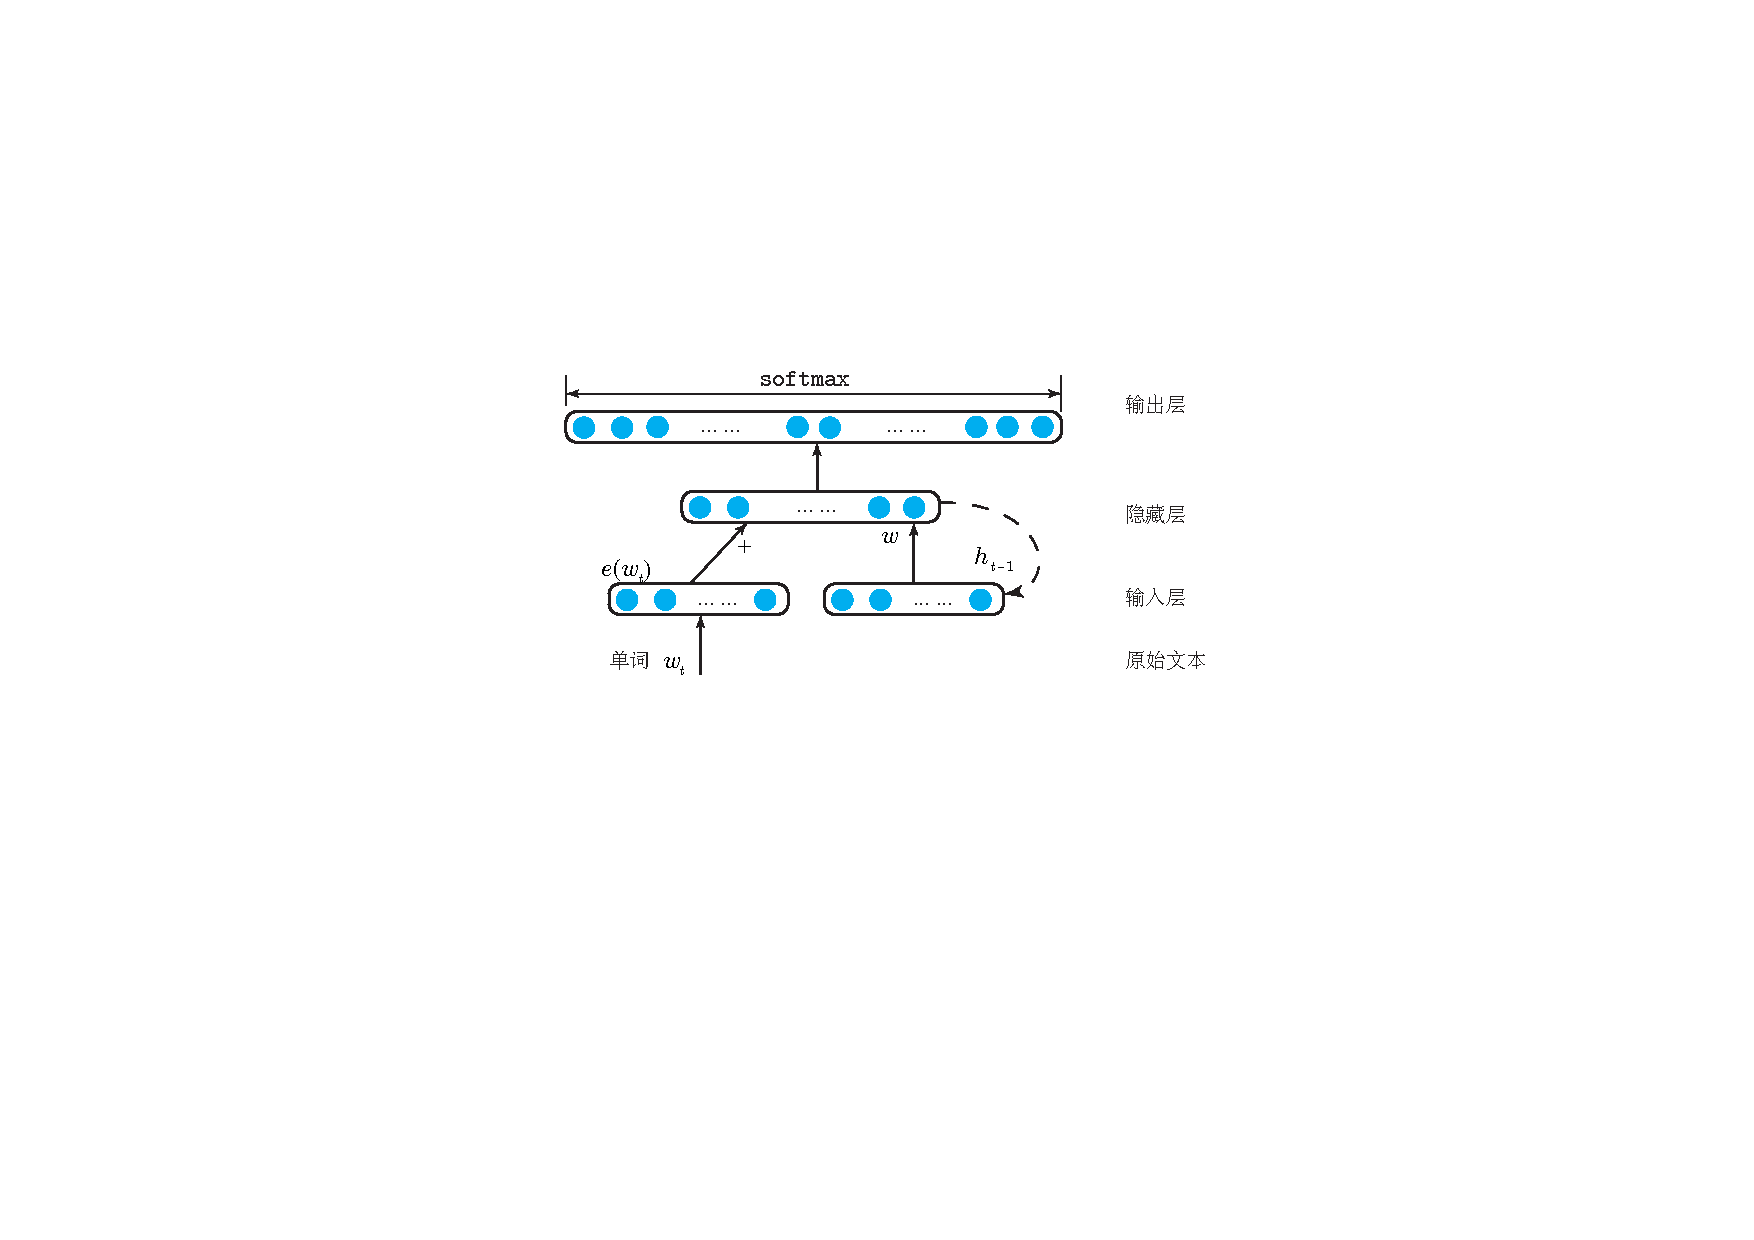
\includegraphics[width=0.85\linewidth]{./figures/rnnlm.png}
  \caption{循环神经网络语言模型(RNNLM)模型结构图}\label{fig:rnnlm}
\end{figure}


\section{关键技术或技术路线}
\subsection{关键技术}

\subsection{技术方案}
\section{论文研究计划}
\begin{itemize}
  \item 2016年12月 $\sim$ 2017年1月: 整理资料,学习研究语言模型的领域知识;
  \item 2017年2月$\sim$ 2017年4月: 研究学习深度学习模型的知识, 特别是循环神经网络的建模过程;
  \item 2017年5月$\sim$2017年7月: 调研并实现解决大词表问题的主要手段, 并实现基本代码框架;
  \item 2015年8月$\sim$2015年10月: 实验验证与完善;
  \item 2015年11月$\sim$2015年12月:资料整理和论文撰写.
\end{itemize}



\newpage
\addcontentsline{toc}{section}{主要参考文献}
\bibliography{bibs}

\end{document}
